%\vspace{-.5cm}
\section{Tool Demonstration}
\label{sec:demo}
%\vspace{-.5cm}
Discuss the main steps of process that needs to be followed for synthezing
and performing the conformance analysis,that are,
%\vspace{-.5cm}
\subsection{Glossary building and terms definition}
%\vspace{-.4cm}
The first step towards writing the controller specifications as a natural
language in \textsf{EARS-CTRL} is to define the glossary terms. 
The user is provided with an editor
(figure~\ref{fig:glossary_def}) to define glossary terms for the following,
1) components that interface with the controller, 2) sensors and actuators those components make available to the controller and 3) rules between
signals definitions.\levi{I am going to split these rules between aliases and
invariants}
%\vspace{-.5cm}
\begin{figure*}[!h]
\centering
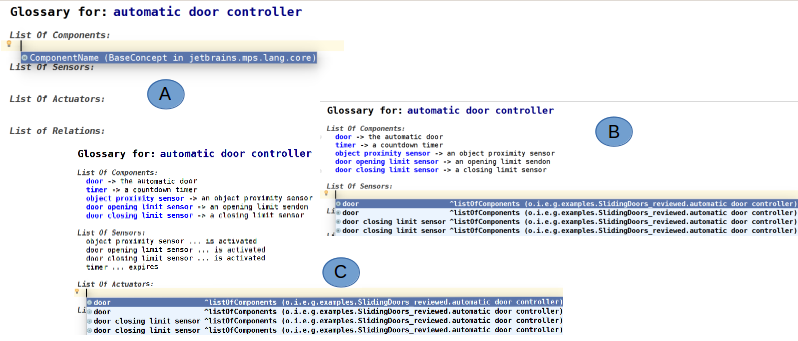
\includegraphics[width=1\textwidth]{./images/glossary_def1.png}
\caption{step-by-step glossary building for sliding door controller: (\emph{A})
Components definition, (\emph{B}) Sensors definition and (\emph{C}) Actuators
definition\levi{be careful with the size of the pictures -- this is not
readable!}}
\label{fig:glossary_def}
\end{figure*}
%\vspace{-2cm}
\subsection{Building \textsf{EARS-CTRL} requirements for the controller}
%\vspace{-.5cm}
The user is provided with an editor built in MPS
is provided to start specifying the controller behavior. The user can input the
requirements simply by filling in the instance of the EARS template with
placeholders in the editor. Figure~\ref{fig:EARS_req} provides step-by-step
guidance to write the EARS requirements. In the projectional editor the user is
provided with the option (i.e., using CTRL+Space keys on keyboard) to intantiate
the EARS-based template with placeholders (\emph{Step A}). After obtaining an
instance of the EARS template, the user starts filling in the placeholders with the information
(i.e., glossary definitions) (\emph{Step B}). \emph{Step C} of the
figure~\ref{fig:EARS_req} depicts a complete sliding door controller specification.
\begin{figure*}[!h]
\centering
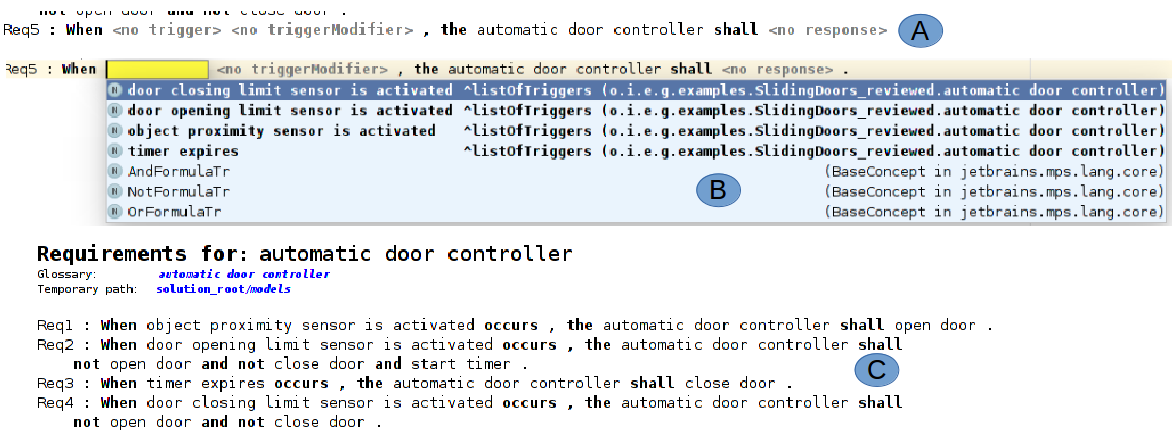
\includegraphics[width=1\textwidth]{./images/EARSREQSPEC.png}
\caption{step-by-step \textsf{EARS-CTRL} for controller requirements: (\emph{A}) Empty
instance of EARS template with placeholders, (\emph{B}) Filling instance of an EARS
template with information and (\emph{C}) Completed EARS Specification }
\label{fig:EARS_req}
\end{figure*}
\subsection{Realizing \textsf{EARS-CTRL} requirements}
%\vspace{-.3cm}
The user of the tool can attempt to realize\levi{I used synthesize on the main
paper, not realize} (by applying the \emph{Transform} intention) the controller
once the controller is completely specified. This will be acheived by applying
the intention (applying\levi{two times ``applying''} \emph{Alt+Enter} keys) on
the root of the specification shown in \emph{part A} of
figure~\ref{fig:Spec_transform}. The generated output of the transformation
comprised of, 1) Controller Holder: Data Flow Diagram with blocks (\emph{part B}
of figure~\ref{fig:Spec_transform}) and 2) Gate Descriptors:
Pseudo code representing the behavior of the blocks (\emph{part C} of
figure~\ref{fig:Spec_transform}).
%\vspace{-.7cm}
\begin{figure*}[!h]
\centering
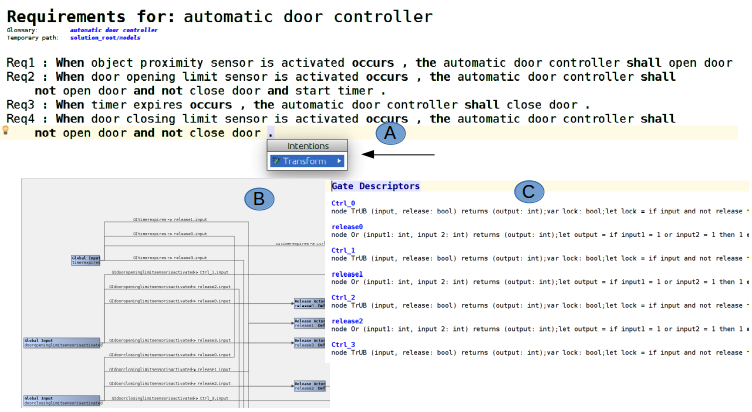
\includegraphics[width=1\textwidth]{./images/Spec_Transform.png}
\caption{Controller generation: (\emph{A}) Applying Intention (Alt+Enter),
(\emph{B}) Data Flow Diagram of the controller (an excerpt) and (\emph{C})
Pseudo code representing the behavior of the blocks (an excerpt)\levi{are the pictures
readable?}}
\label{fig:Spec_transform}
\end{figure*}
\vspace{-1.2cm}
\subsection{Simulation and Test Cases for Analysis\levi{we don't need to go
to the Simulink level (except maybe for code generation??)}} Analysis for
verification of the generated controller with respect to its specification can be performed manually by simulating the behavior in Matlab
Simulink \cite{MatlabSimulink}. The analysis can be performed as follows,
%\vspace{-.5cm}
\subsubsection{Generation of Simulink model}
The user first applies the intention \emph{GenerateSimulinkModel} on the root of
the \emph{Controller Holder} model generated earlier (i.e., part \emph{A} of
figure~\ref{fig:SimulinkModelgeneration}). The result of applying the intention is \emph{.m} Simulink extention file
(i.e., part \emph{B} of figure~\ref{fig:SimulinkModelgeneration}) with Simulink
information for block diagram generation. The user then clicks the Run button
and as a result gets the Simulink block diagram (i.e., part \emph{C} of
figure~\ref{fig:SimulinkModelgeneration}). 
\begin{figure*}[!h]
\centering
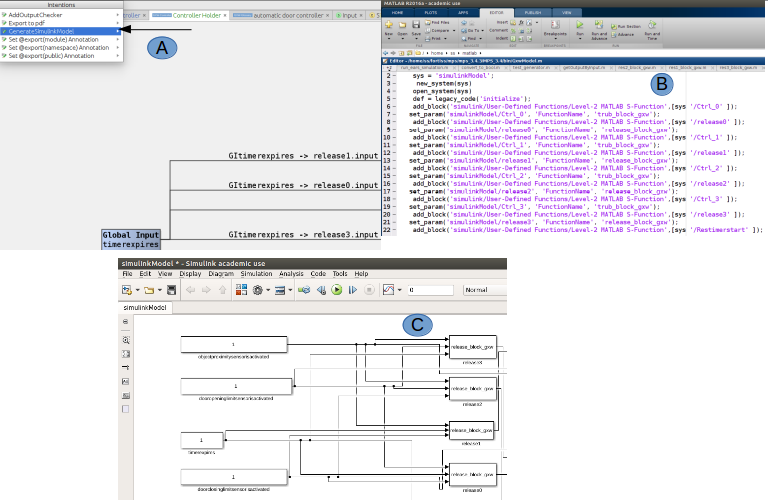
\includegraphics[width=1\textwidth]{./images/SimulinkModelGeneration.png}
\caption{Simulink Model generation for analysis: (\emph{A}) Applying
GenerateSimulinkModel Intention, (\emph{B}) Open generated .m file in Simulink
and (\emph{C}) Generated Simulink block diagram\levi{are the pictures
readable?}}
\label{fig:SimulinkModelgeneration}
\end{figure*}
%\vspace{-.5cm}
\subsubsection{Analysis using Simulation and Test cases\levi{all should be
launched from the MPS IDE}} The user can automatically generate test cases and
simulate the behavior in order to perform the analysis of the controller
(as shown in figure~\ref{fig:SimandAnalysis}). In order to automatically perform
the testing and collecting the simulated data, the user can utilize the Simulink console and execute the following command in the Simulink console
``run\_ears\_simulation 2 false false'' in order to simulate the
controller behavior in Simulink. The result of the simulation is saved as a text file that contains the inputs and generated outputs as a set of sequences. The generated text file is parsed in MPS. Model
is generated in MPS when the user applies the intention \emph{Produce Simulink Result Model}.
\begin{figure*}[!h]
\centering
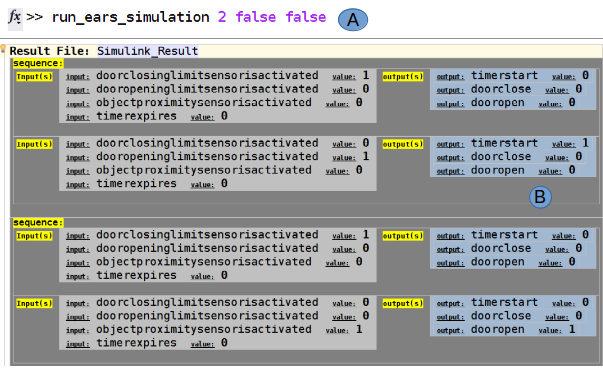
\includegraphics[width=1\textwidth]{./images/Simulation_and_Analysis.png}
\caption{Simulation and Analysis: (\emph{A}) Simulink function to Simulate the
Controller Behavior and (\emph{B}) Model in MPS after parsing the
Simulation results}
\label{fig:SimandAnalysis}
\end{figure*}